% Chapter 6

\chapter{Building a High-fidelity Prototype} % Main chapter title

\label{Building a High-fidelity Prototype} % For referencing the chapter elsewhere, use \ref{Chapter1} 

\lhead{Chapter 6. \emph{Building a High-fidelity Prototype}} % This is for the header on each page - perhaps a shortened title

%----------------------------------------------------------------------------------------

Once the paper prototype was complete, it was converted into a Balsamiq \citep{Balsamiq} mockup (see Figure  \ref{fig:Balsamiq}), to be as tidy and legible as possible, as well as digitally portable. This allowed for easy sharing and backing up (e.g. it could be saved to Dropbox and viewed anywhere, on any device) because it was a small PDF file and not an A2 roll of paper. It also provided a more legible version of the paper prototype that didn't include scratched out notes or other visual ambiguities that could confuse the development process. 

%\begin{figure}[h!]
\begin{sidewaysfigure}
    \centering
    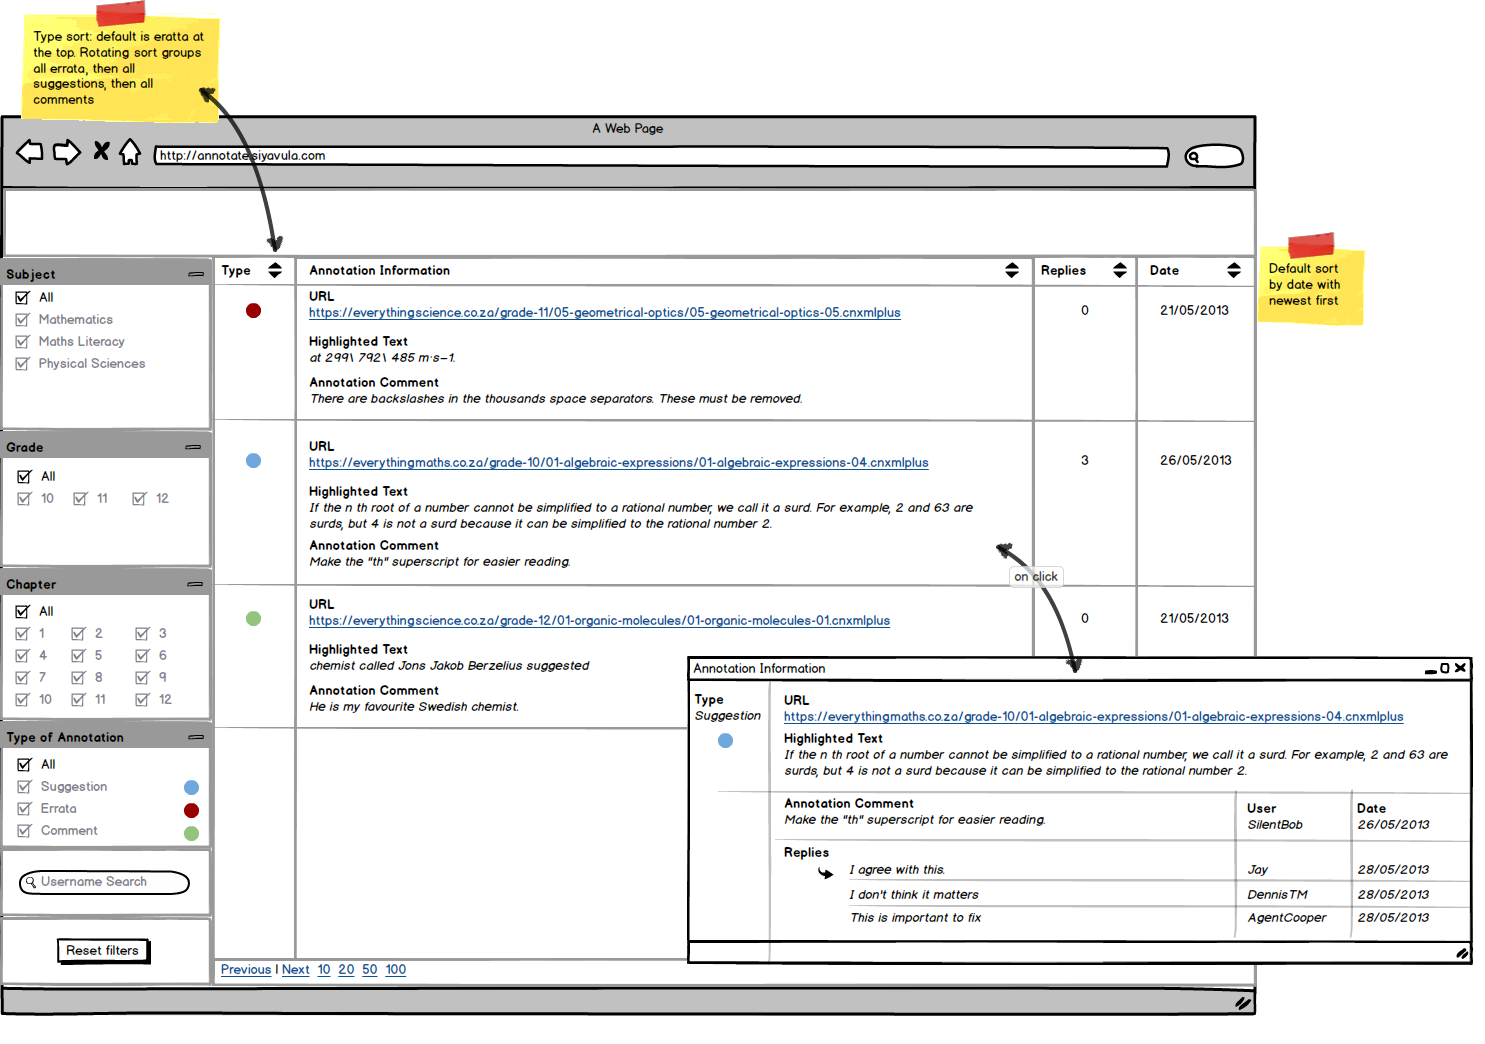
\includegraphics[width=\textwidth]{Figures/BalsamiqMockup.png}
 \caption{Balsamiq mockup of the final paper prototype.}
 \label{fig:Balsamiq}
 \end{sidewaysfigure}
%\end{figure}

This mockup was then converted into a functional, high-fidelity prototype website using HTML, CSS and XML, as is detailed below. Scripted functionality was built using Javascript and the JQuery library in particular.  

The site was hosted using GitHub Pages \citep{GitHub} at \href{http://nicoladt.github.io/MIT-Thesis/}{http://nicoladt.github.io/MIT-Thesis/} which offers simple, free hosting, and seamless integration with GitHub version control software. Assistance was given by Ewald Zietsman with the Javascript and JQuery coding. 

\section{The high-fidelity prototype}



\subsection{Technical details}
The interface was comprised of two main areas (see Figure \ref{fig:HifiMain}). The column on the left contained all the filter options, and the table making up the rest of the page displays the annotations in rows.

Placeholder annotations were made in an XML file. Each annotation was assigned a type and had a simple data structure including a timestamp, a URL (pointing to a particular webpage on the live webbooks sites), a username, highlighted text (from the book), and a user comment. In addition each annotation could have one or more replies. Replies in turn also had a timestamp, username and user comment: 
\begin{verbatim}
<annotation type="">
  <url></url>
  <username></username>
  <datetime></datetime>
  <highlighted></highlighted>
  <comment></comment>
  <replies>
    <reply>
      <username></username>
      <comment></comment>
      <datetime></datetime>
    </reply>
  </replies>
</annotation>
\end{verbatim}

For the prototype, annotations were not given unique ID's or primary keys. Whilst this would be necessary for real annotations (due the the possible complexities of many users making many annotations simultaneously), for the prototype a combination of the URL and timestamp was used as a unique identifying characteristic. 

Annotations were constructed carefully with evaluation tasks in mind. They were created so as to represent at least every possible combination of subject and grade. Annotations were assigned to the three types (comment, errata, suggestion) and random usernames were created. Replies (in number from 1 to 3) were added to some annotations.

The interface was built upon the basic components of the Bootstrap 2.3.2 framework \citep{Bootstrap}. Bootstrap was selected not only because of its built-in cross-browser compatibility but also because it comes packaged with clean and simple CSS and a number of default elements (like buttons) that are easily customizable. 

The DataTables jQuery plugin \citep{DataTables} was implemented for easy control over the table and its functionality and behaviour. 

%\begin{figure}[h!]
\begin{sidewaysfigure}
    \centering
    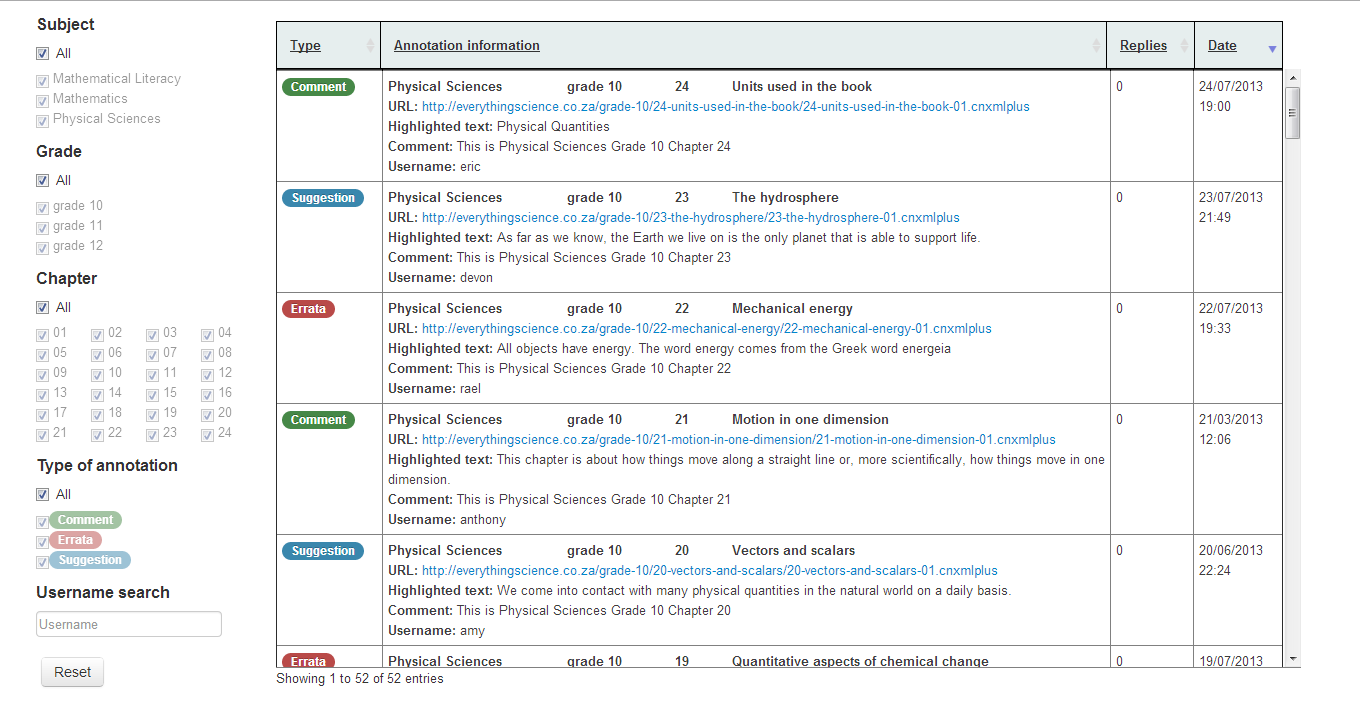
\includegraphics[width=\textwidth]{Figures/V1/HiFi1mainview.PNG}
 \caption{Screenshot of the high-fidelity prototype.}
 \label{fig:HifiMain}
\end{sidewaysfigure}
% \end{figure}

A fixed header for the the table was deemed important, so that users always knew what each column represented. However, DataTables fixed header functionality does not work correctly with pagination (a known bug), so a compromise was reached and vertical scrolling was enabled instead. Pagination breadcrumbs (arguably not necessary for sets of annotations $<$ 100 entries) beneath the table, were substituted with the automatically-updated line of text saying "\textit{Showing xx number of yy entries}", where xx was the number of rows in the table, and yy the total number of annotations (see Figure \ref{fig:breadcrumbs}).

\begin{figure}[h!]
    \centering
    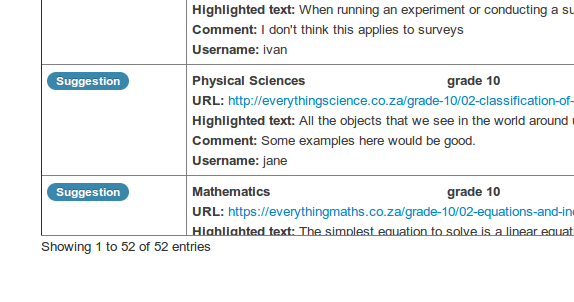
\includegraphics[width=0.7\textwidth]{Figures/V1/breadcrumbs.png}
 \caption{Text beneath the table indicated how many rows (annotations) are surfaced}
 \label{fig:breadcrumbs}
\end{figure}

DataTables also contains an unfortunate (and well-documented) CSS bug, in which the fixed table header \verb|<th>|                                                                                                                cells do not always align correctly with the table data \verb|<td>| cells beneath them. However, this is a minor visual issue concerning a few pixels.

DataTables can only handle an alphabetical sort of columns, which meant that a three-way (rotational) sort of the "type" column was not possible - i.e. it was not possible to sort so that "errata" was listed at the top, "e" being between "c" (comment) and "s" (suggestion) in the alphabet. Additionally, it is only possible to perform a default sort on one column initially, so a sort based on Date and then Type was not possible.

Whilst the loss of these possibilities is noteworthy, it was decided to proceed with the implementation of the DataTables plugin, because the missing functionality could easily be substituted using other techniques (e.g. it was very easy to filter all the annotations by "type" to get to the third sorting category of "errata"). For this reason it was decided that the pros of using the DataTables plugin outweighed these few cons.

Javascript and the jQuery library were chosen to do the information processing required by the interface. jQuery allows for client-side processing. It is simple to implement, and runs as a light-weight instance in any browser \citep{jQuery} \citep{JS}. Practically, client-side data processing (as opposed to HTTP calls to a server) allows for rapid updates to a webpage, and therefore to the interface itself. 

GitHub Pages was selected as the simplest hosting solution for the prototype, because it is secure and reliable, and most-importantly integrates seamlessly with GitHub version control software. However GitHub Pages can only serve static HTML and it cannot handle server calls. Again, the pros of using GitHub Pages outweighed the single loss of functionality it presented, which was the inability to use cookies to store user session information. 


In terms of scripting behaviour, the script written parses the list of XML annotations and builds then builds the filters on the left of the interface based on what it finds in the XML. Each URL from everythingmaths.co.za and everythingscience.co.za contains information about the subject, grade, chapter and section applicable to that annotation. This information is parsed from the URL and presented in a human-readable text format, both as filters on the left-hand side, and as inline text for each annotation. 

\subsection{Behaviour}
Once the filters have been constructed from the XML, the table is then populated based on  the selection filters on the left of the page. The default is that all the annotations are selected and therefore all the annotations are displayed in the table. The basic behavioural pattern is that interacting with the left-hand filters automatically changes what is visible in the table. Any changes made to the left-hand selection cause the table to display only the annotations relevant to the new parameters selected on the left. 

The checkboxes are grouped according to the field \citep[p. 439]{Galitz}: i.e. by subject, grade, chapter number and type. 

Initially the 'All' checkboxes were ticked, and the sub-checkboxes were also ticked but greyed-out, as per the paper prototype. Clicking on a sub-check selected that particular checkbox, deselected the "All" checkboxes and deselected all other sub-checkboxes. It also made the sub-checkboxes opaque (see Figure \ref{fig:checkboxes1}). 

\begin{figure}[h!]
    \centering
    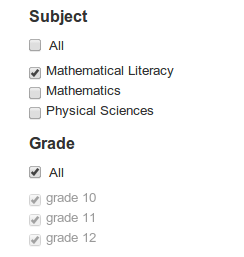
\includegraphics[width=0.4\textwidth]{Figures/V1/checkboxes.png}
 \caption{Single selection of sub-checkbox, compared to selection of "All" checkbox.}
 \label{fig:checkboxes1}
\end{figure}

Clicking on an checked "All" checkbox deselected the "All", selected all of the sub-checkboxes in that filter category, and made them opaque (see Figure \ref{fig:checkboxes2}). In other words, the "All" checkbox behaved as an 'all or subset' toggle, not an 'all or nothing' toggle (which would just result an empty table). 

Whilst this deviated from the standard checkbox behaviour ('all or nothing'), firstly it is the behaviour participants suggested in the design sessions. Secondly \citep[p. 435]{Galitz} this modification allowed for the possibility that a user would want to invert a selection: i.e. to select most (but not all) of the sub-checkboxes in a category. For instance, a user might want to select 23 of of 24 chapter checkboxes. Clicking 23 times would be tedious indeed. With the "All" behaviour described above, a user could simply deselect the "All" checkbox and deselect the chapters they did not want included in the results.

\begin{figure}[h!]
    \centering
    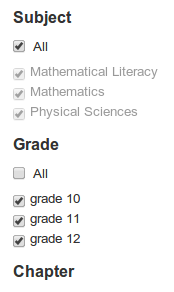
\includegraphics[width=0.3\textwidth]{Figures/V1/alldeselected1.PNG}
 \caption{Subject, with "All" checked vs. Grade, with "All" unchecked and all sub-checkboxes activated.}
 \label{fig:checkboxes2}
\end{figure}

The username search box was a simple, case-sensitive text search. It did not serve up an auto-completing drop-down list. Instead, the table updated automatically (with each new character typed) as the user began typing into the input box. This alternative behaviour to that specified in the paper prototype was selected because it was consistent \citep[p. 261]{DixFinlay} with the behaviour of the table for all other filter fields, whilst still giving users the immediate feedback they required (in the form of instantly updated results with every keystroke) when performing a potentially uncertain search for a username. 

The button labelled "Reset" simply reset the page to the default view (see Figure \ref{fig:reset}). 
\begin{figure}[h!]
    \centering
    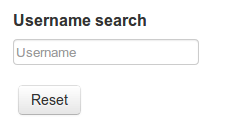
\includegraphics[width=0.4\textwidth]{Figures/V1/usernameReset.png}
 \caption{The username search box and "Reset" button.}
 \label{fig:reset}

\end{figure}

The table was sorted by default by descending date (see Figure \ref{fig:sort}).  As mentioned above, it was not sorted with errata at the top of  the type column due to DataTables' strictly alphanumeric sorting capabilities. That being said, an alternative method for viewing "errata" type annotations at the top of the table was provided by the type filter on the left so this was deemed an acceptable alternative. 
\begin{figure}[h!]
    \centering
    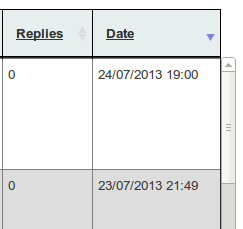
\includegraphics[width=0.35\textwidth]{Figures/V1/sorticons.png}
 \caption{"Sortable" vs "sorted: descending" icons in the table header}
 \label{fig:sort}

\end{figure}	

On mouseover of the table rows, the row changed colour (from white to light grey) and the cursor changed to be a "zoom in" cursor to indicate that action is possible: that the row is clickable and there are more details to be viewed or expanded (see Figure \ref{fig:mouseover}).

\begin{figure}[h!]
    \centering
    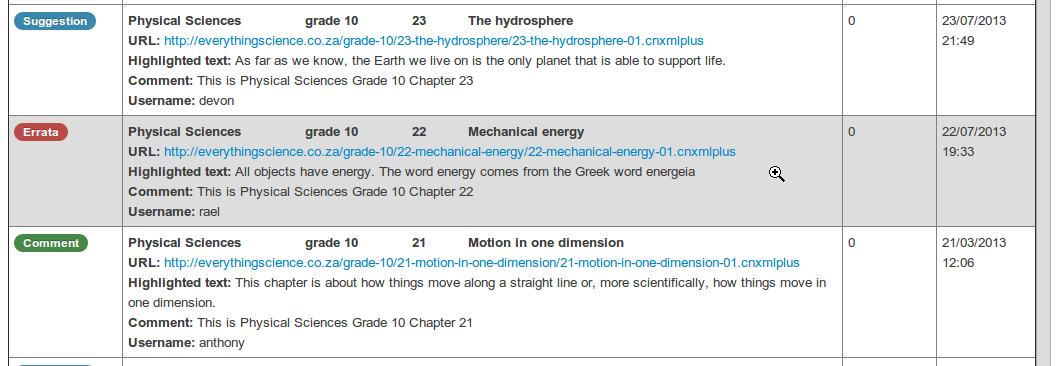
\includegraphics[width=\textwidth]{Figures/V1/mouseover.png}
 \caption{Grey row colour and zoom icon on hover.}
 \label{fig:mouseover}

\end{figure}

Clicking on a particular annotation brought up the detailed view window as an overlay on the table (see Figure \ref{fig:detailedview}). As well as all of the annotation information visible in the table, this view also included all replies to an annotation and the reply details. To close the detailed window, users could click on the [x] in the top right corner of the window or they can press the [Esc] key. 

Because the detailed view was an overlay of the interface and not a separate browser window, a "Back" button (as in the paper prototype) was not included. Users were given two standard alternatives to close the overlay instead. 

\begin{figure}[h!]
    \centering
    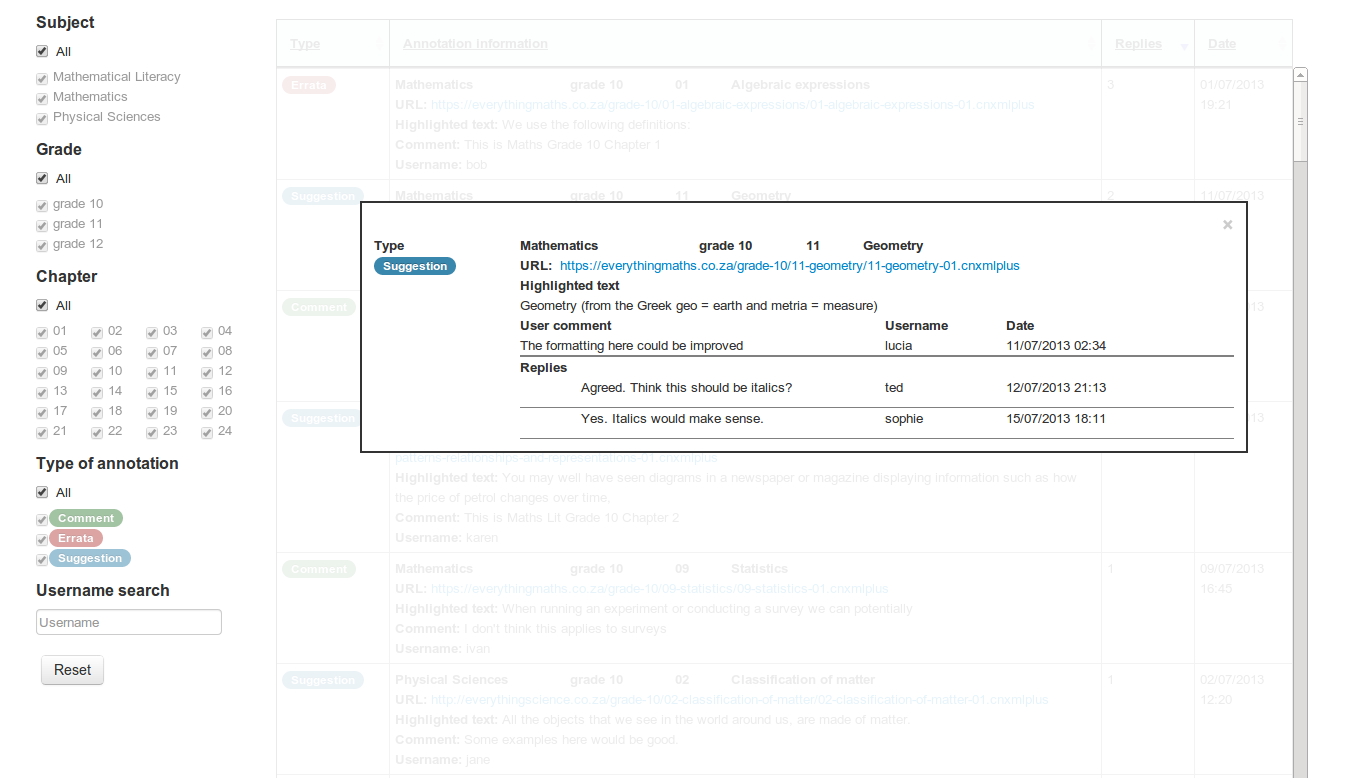
\includegraphics[width=\textwidth]{Figures/V1/detailedview.png}
 \caption{The detailed view overlay.}
 \label{fig:detailedview}

\end{figure}

\section{How and why the high-fidelity prototype differs from the paper prototype}
As mentioned in Chapter 5, certain functionality that was discussed in the paper prototyping process was excluded because it required the integration of server-side processing and issue tracking software, which would significantly extend the scope of the system. Differences between the paper and high-fidelity prototypes are detailed as follows. 
\begin{enumerate}
 \item \textbf{No cookies}\\
For simplicity of development and in order to use GitHub Pages for hosting, the interface only used client-side processing, without any server integration. This meant that cookies to store information about a user's session could not be saved and that if a user navigated away from, and back to the webpage, it would be reset to its default view: the user's last filter selection would not be saved. \\
\\
The advantages gained by using GitHub were significant, as mentioned already. Additionally, it could be argued that the selection of filters and live updating of the resulting table was simple and quick enough that redoing a task would be relatively trivial. 

\item \textbf{No user authentication}\\
Again, because of the lack of a server, user authentication was not implemented in this prototype. Authentication is arguably not needed to test the interface functionality itself however: it would be an independent process that would take place in its entirety before a user came to view the interface in question. 

\item \textbf{No collapsible filters}\\
The groups of filters and checkboxes were not collapsible, because they all fitted onto one page. The collapsibility was suggested by users during the paper prototyping sessions because they were concerned that there would be too much information to fit onto one webpage. In implementation however, this was not the case, so this functionality was set aside. Because the filters offer a graphical representation of the system status (what is visibly selected on the left maps directly to what information is in the table) displaying all filters on one page also improved observability \citep[p. 270]{DixFinlay} for users.

\item \textbf{No username auto-complete suggestions}\\
The username search box did not offer a drop-down list of auto-complete suggestions when users started typing. Instead, it updated the table of results automatically with each keystroke. This behaviour was the same as for all the other filter categories, and so it replicated a pattern found throughout the interface (consistency and predictability), while still giving users immediate feedback (instantaneous responsiveness) and the easy ability to undo actions (recoverability) \citep[p. 272]{DixFinlay}. 

\item \textbf{Extra information added to each annotation cell}\\
At the top of each "Annotation Info" cell, a line of bold text containing the subject, grade, chapter number and chapter name was added to give users more  easily readable information about where each annotation was from, so they did not have to decipher a long URL.

\item \textbf{No back button in detailed view}\\
Because the detailed view was an overlay and not a new webpage a "Back" button was not included (users making the prototype specified that the detailed view should open in the same page). Instead, users could close the overlay by clicking on the [x], in the top right corner, or by pressing the [Esc] key - both standard interface patterns \citep[p. 345]{Galitz}. Using an overlay instead of a new webpage or window also prevented users from leaving the webpage unnecessarily, and therefore reduced the risk of users getting lost in a navigation process. 

\item \textbf{No Life Sciences subject}\\
Due to external factors, the Life Sciences Grade 10 book was not yet available on the Everything Science website, so it was excluded because there were no live URLs available for that content. 

\item \textbf{No curriculum alignment filter}\\
By the time the high-fidelity prototype was being built, all available textbooks on the Everything Maths and Science websites were aligned to the current CAPS curriculum, and no old NCS content was available. Hence, the curriculum alignment filter was excluded. 

\item \textbf{Lower-level filters do not update}\\
Participants in the design sessions suggested that lower-level filters (like chapter) should update based on the higher selection. I.e. the list of grade filters would update depending on the subject choice, and the number of chapters would change to reflect what was available in a specific combination of grade and subject. \\
\\
If users performed a unidirectional filter operation this functionality would be useful. However excluding it and displaying all possible subjects, grades and chapters meant that users could easily change their selection, and filter both forwards and backwards. This made it far simpler to correct mistakes, undo actions or browse the data and discover new information, all of which conforms to good design principles \citep[p. 272]{DixFinlay}. \\
\\
Additionally, displaying all of the possible filters at once meant that users always have visual feedback about what they \textit{had} selected, in the context of what they \textit{could} select. This would make current and future states more apparent and discoverable (which ties into the design principle of observability \citep[p. 270]{DixFinlay}).  

\item \textbf{No coloured dots next to "Type"}\\
The coloured circle icons suggested for "Type" categories were replaced by coloured labels beneath the "Type" text.  These coloured labels are packaged as part of the default Bootstrap styles, and were therefore simplest to implement, the visual  effect arguably being the same. Three colours were selected based on users' paper prototype suggestions, available Bootstrap label colours and common meanings for colour \citep[p. 635]{Galitz} (e.g. red, which often signifies a warning was used for errata).

\item \textbf{No right-clicking of rows}\\
Right-clicking an annotation row did not open it in new tab. This was simply because the detailed view was constructed as a visual overlay, and not as a new webpage. 

\item \textbf{DataTables-related changes}
  \begin{enumerate}
    \item \textbf{No double default sort}\\
    As discussed above, using DataTables meant that it was not possible to perform a default sort by date \textit{and} type. Because of the ease with which users could filter by type on the left-hand side of the interface, the default sort was simply by date, descending. 
    \item \textbf{No breadcrumbs or pagination}\\
    Due to DataTables' fixed table header not working with the built-in pagination functionality, pagination was substituted with vertical scrolling. Instead of "Previous $\vert$ Next $\vert$ 10 $\vert$ 20 $\vert$ 50 $\vert$" breadcrumbs at the bottom a message was surfaced indicating how many annotations (rows) were displayed in the current table.
    \item \textbf{Strict alphanumeric sorts}\\
    Because DataTables' sorting functionality is strictly alphabetical, a three-way sort for the type column (to surface "errata" at the top) was not possible. Similarly, the annotation information column could not be sorted by URL. Instead it was sorted by the subject, grade and chapter number text at the top of each cell (the same information that the URL provided anyway). 
  \end{enumerate}
  
\end{enumerate}

\section{Discussion}
Whilst the high-fidelity prototype did diverge from the paper prototype slightly, wherever possible behaviour or design specified in the paper prototype that could not be included was substituted with an equivalent solution. Trade-offs (e.g. using DataTables) were carefully evaluated so that whenever possible, more functionality was gained than was lost or had to be altered. 

Any divergence could (and would) also be thoroughly evaluated by users in the next part of the process, involving usability testing and formative evaluation. 

In some cases, the implementation of the prototype in an actual web browser opened up new possibilities - such as styling the filters to all fit on one standard 1366 x 768 resolution screen. The visual effects of an overlay are also easier to envision and explore with HTML and CSS than on paper. 

Several aspects of the high-fidelity prototype were not highly scalable. For example, client-side processing of thousands (not dozens) of annotations in future would get extremely slow. Similarly, while reloading the table with a few annotations takes only milliseconds, with a large database of annotations, and a more complex set of filters (e.g. more subjects, more grades) the load time would be significantly increased. There is no doubt a performance threshold at which it would become practical to implement server-side processing instead, which would also mean that user authentication and use of cookies would become possible. Similarly, with a larger database, pagination of the table (with breadcrumbs) as opposed to vertical scrolling would be necessary to reduce load and response time of the interface. 

Whilst DataTables provided a lot of pre-packaged functionality, it is currently not very robust, and it appears that new releases and improvements, while pending, are slow to occur. Ideally it would be better to reinvent the wheel, and write customised code to handle sorting (e.g. three way sort, implementing more than one default sort parameter), pagination, header behaviour and so on. 

Once the high-fidelity prototype of the interface was complete the next step was to formatively evaluate it with a new group of users \citep[p. 329]{RogersPreece}, to ensure that the design thus far still conformed to user requirements and expectations. Once this was done, the interface could then be iteratively improved based on the first round of usability tests and user feedback. This process of evaluation and iteration will be discussed at length in the next chapter. 
